\chapter{CHAPTER FOUR: FINDINGS} \label{chapter_4}


Chapter Four, also called �Results� or �Data Analysis,� usually provides detailed findings of the research. This chapter is where tables and figures most often appear, so make sure formatting is consistent.

\section{Sample Table}

The following sample table is an example of acceptable table formatting. Descriptive titles appear above tables and may appear either on one line or stacked and single-spaced. The table itself may also be single-spaced as necessary.
If possible, try to keep tables and/or figures all on one page. If necessary, start the table or figure on a new page, even if this means leaving blank space on the preceding page. If you must split a table over multiple pages, repeat the table headings and continue. It is not necessary to repeat the table title.

\begin{table}[!ht] \singlespacing
\caption{Classroom Checklist for Physical Organization (a sample table)} \label{tbl:my_first_table}
\begin{center}
\begin{tabular}{lcccccc}
 & \multicolumn{6}{c}{Classrooms} \\ \hline
Physical Components & A & B & C & D & E & F \\
Desk Groupings for Student Interaction & 5 & 3 & 3 & 5 & 3 & 2 \\
Learning and Resource Centers & 3 & 2 & 2 & 3 & 1 & 1 \\
Flexibility of Furniture Use & 3 & 4 & 3 & 3 & 2 & 1 \\
Specific M/G Displays & 1 & 1 & 3 & 2 & 2 & 2 \\
Total out of 30 points & 12 & 10 & 11 & 13 & 8 & 6 \\ \hline
\end{tabular}
\end{center}
\vspace{-4ex}
\begin{minipage}{\textwidth}
\singlespacing \footnotesize \flushleft
Degree of Application: 5=High; 4=Medium-High; 3=Medium; 2=Medium-Low; 1=Low
M/G=Multicultural/Global

\noindent A, B, C, D, E, and F are the classrooms of Alice, Betty, Carol, Donna, Elaine, and Fran respectively.
\end{minipage}
\end{table}

\section{Sample Figure}

The following is a sample figure with acceptable figure formatting. For figures, be sure you format both the figure and the figure title consistently. This includes placement (centered or left-justified), spacing before and after, line spacing, point size and font.

\begin{figure}[!ht] \singlespacing
\begin{center}
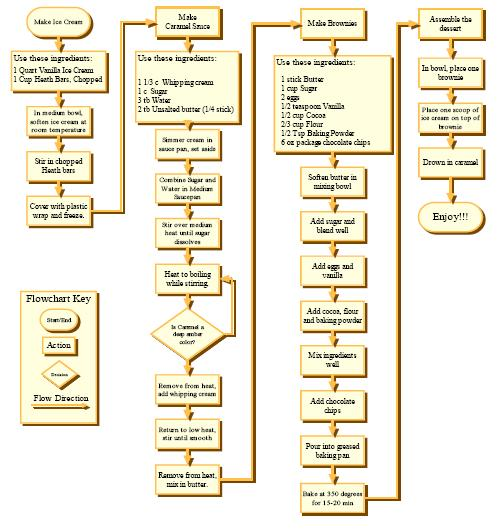
\includegraphics[width=.8\textwidth]{figures/figure_1}  %% good idea to keep your figures in a separate folder
\end{center}
\caption{Heath Bar Caramel Brownie Sundae} \label{tbl:my_first_figure}
\end{figure}

%% Best way to generate pictures, especially graphs, is to save them (say from MATLB) as .eps (Encapsulated PostScript) and than
%% convert to PDF using (attached) eps2pdf utility. Note that pdfTeX will not accept .eps files.